\section{Model Transformations for \SLCO}
\label{sec:reusable-correct-transformations:model_transformations}
DMSLs allow designers to reason at a high level of abstraction, and therefore, DSML models do not include many implementation details.
The main goal of refining model transformations is to add more details to the model, thus bringing it closer to its implementation.
To generate code (such as an \NQC executable) from an \SLCO model, a number of endogenous model transformations have been designed and implemented.
By design, each model transformation transforms only a specific small part of the input model, because small transformations can be easily applied, composed, implemented, and analyzed.
We have composed sequences of transformations for several target languages.
Our correctness criterion guarantees that every intermediate model, including the last model in the sequence, has the same properties as the source model.
Furthermore, the transformations are designed and composed such that the very last \SLCO model in the chain contains all implementation details.

\subsection{Reusability of Model Transformations}
\label{subsec:reusable-correct-transformations:reusability}
Table~\ref{tab:endogenous_model_transformations} lists eleven of thirteen endogenous model transformations that are defined to refine \SLCO models.
The other two transformations deal with time and are not discussed in this chapter.
A detailed discussion of all these transformation is given in Section~\ref{sec:slco:endogenous}.

There are two ways in which these transformations can be reused.
First, a model transformation can be applied multiple times within the same sequence of transformations, as indicated in the second column of Table~\ref{tab:endogenous_model_transformations}.
In practice, the most reused model transformations are the \emph{Clone Classes} transformation, which can be used to clone certain classes, and the \emph{Remove Classes} transformation, which can be used to remove all classes that have no instances.
They ensure that models adhere to the constraints imposed by most of the other transformations and are therefore crucial for the successful composition of transformations.
Second, a model transformation can be applied in multiple sequences leading to different target languages, as indicated in the third column.
This type of reuse is less common, but supporting other target languages with similar semantic gaps would automatically lead to more reuse.
The fourth column is discussed in Section~\ref{sec:reusable-correct-transformations:correctness_of_transformations}.
It shows the number of proof obligations that must be handled to prove the correctness of each transformation.

\begin{table*}[hbt]
\centering
\begin{tabular}{|l|c|c|c|}
\hline
\rowcolor[gray]{.9}
                                          & \textbf{Reused within} & \textbf{Reused for different} & \textbf{Number of proof} \\
\rowcolor[gray]{.9}
\multirow{-2}{*}{\textbf{Transformation}} & \textbf{sequences}     & \textbf{target languages}     & \textbf{obligations} \\
\hline
Bidirectional to                          & \mr{2}{no}             & \mr{2}{yes}                   & \mr{2}{1} \\
Unidirectional                            &                        &                               & \\
\hline
Clone Classes                             & yes                    & yes                           & 1 \\
\hline
Exclusive Channels                        & yes                    & no                            & 1 \\
\hline
Identify Channels                         & no                     & no                            & 1 \\
\hline
Lossless to Lossy                         & no                     & no                            & 74 \\
\hline
Merge Channels                            & no                     & no                            & 1 \\
\hline
Merge Objects                             & yes                    & no                            & 13 \\
\hline
Names to Arguments                        & no                     & no                            & 1 \\
\hline
Remove Classes                            & yes                    & yes                           & 1 \\
\hline
Strings to Integer                        & yes                    & no                            & 1 \\
\hline
Synchronous to                            & \mr{2}{no}             & \mr{2}{no}                    & \mr{2}{4 and 34} \\
Asynchronous                              &                        &                               & \\
\hline
\end{tabular}
\caption{Endogenous model transformations}
\label{tab:endogenous_model_transformations}
\end{table*}

Because of their size and complexity, it is not possible to consider all transformations from Table~\ref{tab:endogenous_model_transformations}.
Instead, we select the two variants of the \emph{Synchronous to Asynchronous} transformation to illustrate our approach.
The difference in complexity of these two variants illustrates that more generic transformations employ more involved communication protocols for handling the introduced changes.
One should search for the strongest possible constraints on the input models for such a transformation~\cite{SLCOexploring2011}.
These constraints shall be realized in separate transformation steps that precede the more complex one in the transformation chain.
This way, many unnecessary details are removed from the core part of the transformation.
The simple variant of the \emph{Synchronous to Asynchronous} transformation also described below, although simple, is still complex enough to illustrate all the  details of our approach.

\subsection{Refining Synchronous Communication}
\label{subsec:reusable-correct-transformations:sync_to_async}
Synchronous communication is a typical example of a construct at a high level of abstraction that is often present in formal modeling languages.
General-purpose programming languages, however, do not offer this concept.
While \SLCO allows for syn\-chro\-nous communication, the communication between controllers on the Lego Mindstorms platform is asynchronous.
Therefore, synchronization should be realized with asynchronous interaction, introduced by correctly defined model transformations built around a properly defined communication protocol.

\clearpage

We defined two different transformations, \TSim and \TGen, to replace one of the synchronous channels in a model by an asynchronous channel.
To keep the observable behavior of the modeled system intact, this change requires and triggers further changes of the related classes, state machines, and transitions.
Transformation~\TSim applies to a restricted subset of models, but is simple and does not greatly increase the complexity of the produced model.
In contrast, transformation~\TGen can be applied to any \SLCO model, but as a more complex protocol is introduced by the transformation, it adds more complexity to the produced model.

Both transformations require the following two constraints to hold for their input.
First, the objects that communicate via the synchronous channel must be the only instances of their classes.
Second, only a single pair of state machines from the two classes may communicate over the channel.
We stress, however, that this does not limit their applicability.
By means of the \emph{Exclusive Channels} and \emph{Clone Classes} transformations, any \SLCO model can be transformed into a model with equivalent behavior that meets these constraints.
Thus, instead of having more complicated transformations that first change models to meet these constraints and then replace synchronous communication by asynchronous communication, we opt for sequences of simpler transformations that have the same effect.
The fact that the constraints hold can be used in the correctness proof of \TSim and \TGen, which greatly simplifies these proofs.

In the remainder of this section, we provide a short description of the aforementioned transformations.
An informal description is given in Section~\ref{subsubsec:slco:sync2async}, and a more detailed description is given in Appendix~\ref{ap:transformations-slco}.
For the rest of the section, we assume that in the model~$m$,
the synchronous channel $\it{ch}_s = \it{chn}()~\textbf{sync from}~\it{on_1}.\it{pn_1}~\textbf{to}~\it{on_2}.\it{pn_2}$ is to be replaced with an asynchronous one.
Let object~$o_i$ with name~$\it{on_i}$ be an instance of class~$\it{cl_i}$ with name~$\it{cn_i}$ in model~$m$, for $i=1,2$.
We also assume, as explained above, that object~$o_i$ is the only instance of class~$\it{cl_i}$ and that state machine~$\it{sm_i}$ with name~$\it{smn_i}$ is the only state machine in~$\it{cl_i}$ that uses channel~$\it{ch_s}$, for $i=1,2$.
Furthermore, we use $\it{tr_s} = \it{tn_s}~\textbf{from}~\it{ss_1}~\textbf{to}~\it{ss_2}~\textbf{send}~\it{sgn}()~\textbf{to}~\it{pn_1}$ to denote a transition
of $sm_1$ of $cl_1$ that sends signals over~$\it{ch_s}$ and $\it{tr_r} = \it{tn_r}~\textbf{from}~\it{sr_1}~\textbf{to}~\it{sr_2}~\textbf{receive}~\it{sgn}()~\textbf{from}~\it{pn_2}$ to denote a transition of $sm_2$ of $cl_2$ that receives signals over~$\it{ch_s}$.
Due to the uniqueness of the channel name and the aforementioned constraints, the transformation of the channel $\it{ch_s}$ induces a transformation of the classes $cl_1$ and $cl_2$ only.
We show only the transformation of signals without arguments, but an extension to general signals is straightforward.
In the remainder of this chapter, we deal with simplified \SLCO models, as described in Section~\ref{sec:SLCO:simplified_slco}.


\subsubsection{Simple Transformation}
Transformation \TSim modifies state machines by replacing some of their transitions.
No essential changes are made to the other structures of a model.
It is only applicable if, for every transition~$\it{tr_s}$, there is no other transition with the same source state.
For every transition~$\it{tr_s}$ of $\it{sm_1}$ and for every transition $\it{tr_r}$ in $\it{sm_2}$, we define

\[
\begin{array}{l}
\TSim(\it{tr_s}, \it{pn_1}) = \langle \\
\quad \it{ss_{nw}}, \\
\quad \it{tn_s^1}~\textbf{from}~\it{ss_1}~\textbf{to}~\it{ss_{nw}}~\textbf{send}~\it{ssgn}()~\textbf{to}~\it{pn_1} \\
\quad \it{tn_s^2}~\textbf{from}~\it{ss_{nw}}~\textbf{to}~\it{ss_2}~\textbf{receive}~\it{asgn}()~\textbf{from}~\it{pn_1} \\
\rangle
\end{array}
\]

\[
\begin{array}{l}
\TSim(\it{tr_r}, \it{pn_2}) = \langle \\
\quad \it{sr_{nw}}, \\
\quad \it{tn_r^1}~\textbf{from}~\it{sr_1}~\textbf{to}~\it{sr_{nw}}~\textbf{receive}~\it{ssgn}()~\textbf{from}~\it{pn_2} \\
\quad \it{tn_r^2}~\textbf{from}~\it{sr_{nw}}~\textbf{to}~\it{sr_2}~\textbf{send}~\it{asgn}()~\textbf{to}~\it{pn_2} \\
\rangle,
\end{array}
\]

\noindent
where $\it{ss_{nw}}$ and $\it{sr_{nw}}$ are fresh state names, $\it{tn_s^1}$, $\it{tn_s^2}$, $\it{tn_r^1}$, and $\it{tn_r^2}$ are fresh transition names, $\it{ssgn} \equiv ``s\_"+sgn$, and $\it{asgn} \equiv ``a\_"+sgn$.
In the transformed model, the new states are added to the appropriate state machines, and the transitions~$\it{tr_s}$ and~$\it{tr_r}$ are replaced by the newly generated transitions.
For ease of reference, a graphical representation of the states and transitions in the definition above is given in Figure~\ref{fig:reusable-correct-transformations:trans_simple}.

\begin{figure}[hbt]
  \centering
  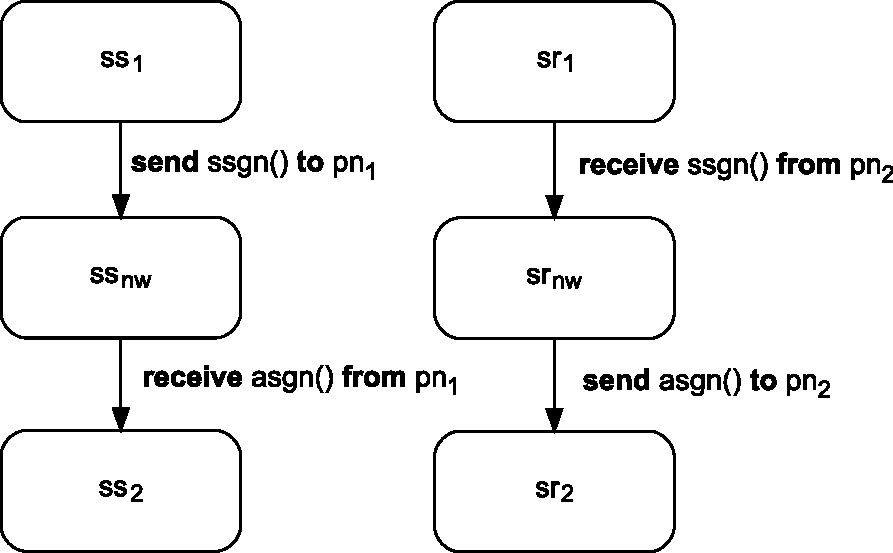
\includegraphics[scale=0.45]{reusable-correct-transformations/figs/transformation_simple}
  \caption{Partial state machines that illustrate \TSim}
  \label{fig:reusable-correct-transformations:trans_simple}
\end{figure}

\subsubsection{General Transformation}
Transformation \TGen is more general than \TSim, due to which it adds more complexity to the produced model.
In this case, also classes are transformed, and new state machines are created.
The restrictions we had on \TSim are removed, which means that \TGen can be applied to any $\it{tr_s}$ of $\it{sm_1}$ and any $\it{tr_r}$ of $\it{sm_2}$ as defined above.
Transformation~\TGen on transitions is defined as

\[
\begin{array}{l}
\TGen(\it{tr_s}, \it{pn_1}, \it{vc_1}) = \langle \\
\quad \it{ss_3}~\it{ss_4}~\it{ss_5}~\it{ss_6}~\it{ss_7}, \\
\quad \it{ts_1}~\textbf{from}~\it{ss_1}~\textbf{to}~\it{ss_3}~\it{vc_1}==0 \\
\quad \it{ts_2}~\textbf{from}~\it{ss_3}~\textbf{to}~\it{ss_4}~\textbf{send}~\it{sgn}(1)~\textbf{to}~\it{pn_1} \\
\quad \it{ts_3}~\textbf{from}~\it{ss_4}~\textbf{to}~\it{ss_5}~\it{vc_1}==2 \\
\quad \it{ts_4}~\textbf{from}~\it{ss_5}~\textbf{to}~\it{ss_6}~\textbf{send}~\it{sgn}(3)~\textbf{to}~\it{pn_1} \\
\quad \it{ts_5}~\textbf{from}~\it{ss_6}~\textbf{to}~\it{ss_2}~\it{vc_1}==0 \\
\quad \it{ts_6}~\textbf{from}~\it{ss_7}~\textbf{to}~\it{ss_1}~\textbf{send}~\it{sgn}(4)~\textbf{to}~\it{pn_1} \\
\quad \it{ts_7}~\textbf{from}~\it{ss_4}~\textbf{to}~\it{ss_7}~\it{vc_1}:=2 \\
\rangle
\end{array}
\]

\[
\begin{array}{l}
\TGen(\it{tr_r}, \it{pn_2}, \it{vc_2}) = \langle \\
\quad \it{sr_3}~\it{sr_4}~\it{sr_5}~\it{sr_6}~\it{sr_7}, \\
\quad \it{tr_1}~\textbf{from}~\it{sr_1}~\textbf{to}~\it{sr_3}~\it{vc_2}==1 \\
\quad \it{tr_2}~\textbf{from}~\it{sr_3}~\textbf{to}~\it{sr_4}~\textbf{send}~\it{sgn}(2)~\textbf{to}~\it{pn_2} \\
\quad \it{tr_3}~\textbf{from}~\it{sr_4}~\textbf{to}~\it{sr_5}~\it{vc_2}==3 \\
\quad \it{tr_4}~\textbf{from}~\it{sr_5}~\textbf{to}~\it{sr_2}~\textbf{send}~\it{sgn}(0)~\textbf{to}~\it{pn_2} \\
\quad \it{tr_5}~\textbf{from}~\it{sr_4}~\textbf{to}~\it{sr_1}~\it{vc_2}==4 \\
\quad \it{tr_6}~\textbf{from}~\it{sr_7}~\textbf{to}~\it{sr_1}~\textbf{send}~\it{sgn}(0)~\textbf{to}~\it{pn_2} \\
\quad \it{tr_7}~\textbf{from}~\it{sr_6}~\textbf{to}~\it{sr_7}~\it{vc_2}:=3 \\
\quad \it{tr_8}~\textbf{from}~\it{sr_1}~\textbf{to}~\it{sr_6}~\it{vc_2}==4 \\
\rangle,
\end{array}
\]

\noindent
where $\it{ss_j}$ and $\it{sr_j}$, and $\it{ts_j}$ and $\it{tr_k}$ are fresh state and transition names, for~$j=3,\ldots,7$ and~$k=3,\ldots,8$.
Variables~$\it{vc}_1$ and $\it{vc}_2$ are discussed below.
A graphical representation of the states and transitions in the definition above is depicted by the two partial state machines on the left of Figure~\ref{fig:reusable-correct-transformations:trans_general}.

\begin{figure}[hbt]
  \centering
  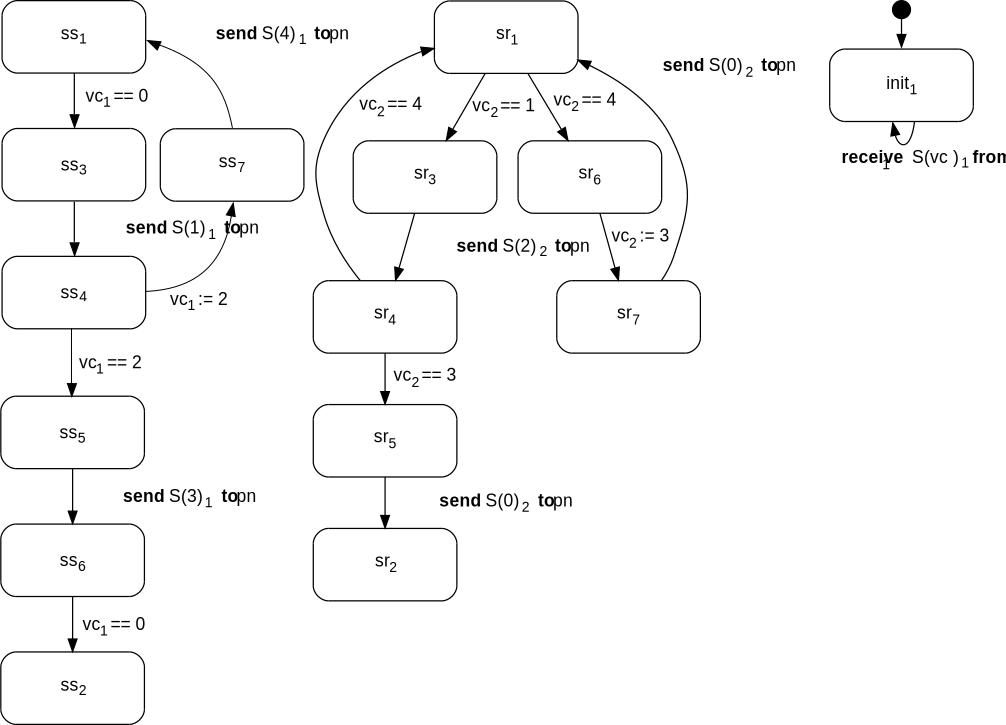
\includegraphics[scale=0.45]{reusable-correct-transformations/figs/transformation_general}
  \caption{Partial state machines that illustrate \TGen}
  \label{fig:reusable-correct-transformations:trans_general}
\end{figure}

In the transformed model, the new states are added to the appropriate state machines, and transitions~$\it{tr_s}$ and~$\it{tr_r}$ are replaced by the new transitions.
Additionally, a fresh integer variable~$\it{vc_i}$ and a state machine~$\it{reader_i}$ are added to the classes~$\it{cl_i}$, for~$i=1,2$.
Let $\it{Tr^G_i}$ be the sets of all $\it{tr_s}$ and $\it{tr_r}$-like transitions of $sm_i$, for~$i=1,2$,
$\it{Sgn_1}$ the set of all signal names occurring in the sending statements of transitions in $\it{Tr^G_1}$,
and $\it{Sgn_2}$ the set of all signal names occurring in the reception statements of transitions in $\it{Tr^G_2}$.
State machine~$\it{reader_i}$ is a result of applying function~$\it{Rsm}$, defined as
%
\begin{align*}
\it{Rsm} & (\it{pn_i}, \it{vc_i}, \it{Sgn_i}) = \it{reader_i}~\textbf{initial}~\it{init_i} \\
& [\it{tsgn_i}~\textbf{from}~\it{init_i}~\textbf{to}~\it{init_i}~\textbf{receive}~\it{sgn}(\it{vc_i})~\textbf{from}~\it{pn_i}~|~ sgn\in Sgn_i],
\end{align*}
%
\noindent
where $\it{reader_i}$ is a fresh state machine name, $\it{init_i}$ is a fresh state name, and $tsgn \equiv ``t\_"+sgn$.
As defined, state machine~$\it{reader_i}$ has a transition for every signal name $\it{sgn}$ from $\it{Sgn_i}$.
On the right of Figure~\ref{fig:reusable-correct-transformations:trans_general}, an example of such a state machine is shown.
